\clearpage
\scanpage{5}
\figure{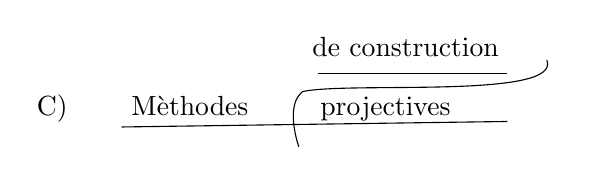
\begin{tikzpicture}[every node/.style={anchor=base west}]
\node at (0,0) {C)};
\node at (1.2,0) {Mèthodes};\node at (3.6,0) {projectives};
\node at (3.5,.75) {\inserted{de construction}};
\draw (1.2,-.15)--(6.1,-.08);\draw (3.7,.53)--(6.1,.53);
\draw (6.6,.7)..controls (6.8,.2) and (4.1,.43)..(3.5,.3)..controls (3.3,.15) and (3.4,-.25)..(3.45,-.4);
\end{tikzpicture}}

\S\,14\quad Familles limitées.

\figure{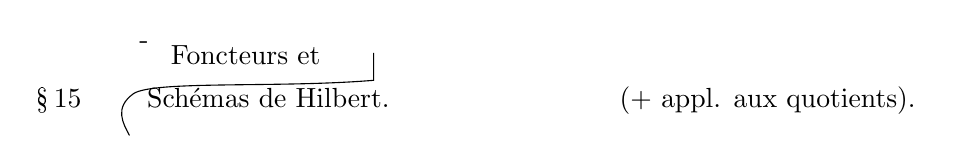
\begin{tikzpicture}[every node/.style={anchor=base west}]
\node at (0,0) {\S\,15};\node at (1.4,0) {Schémas de Hilbert.};\node at (7.4,0) {(+ appl. aux quotients).};
\node at (1.7,.55) {\inserted{Foncteurs et}};\node at (1.3,.75) {\unsure{-}};
\draw (4.4,.7)--(4.4,.35)..controls (3.2,.25) and (1.6,.35)..(1.35,.18)..controls (1.1,0) and (1.22,-.2)..(1.3,-.35);
\end{tikzpicture}}

\figure{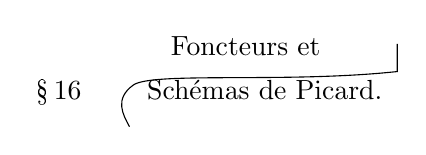
\begin{tikzpicture}[every node/.style={anchor=base west}]
\node at (0,0) {\S\,16};\node at (1.4,0) {Schémas de Picard.};
\node at (1.7,.55) {\inserted{Foncteurs et}};
\draw (4.7,.7)--(4.7,.35)..controls (3.3,.2) and (1.6,.35)..(1.35,.18)..controls (1.1,0) and (1.22,-.2)..(1.3,-.35);
\end{tikzpicture}}
\margin{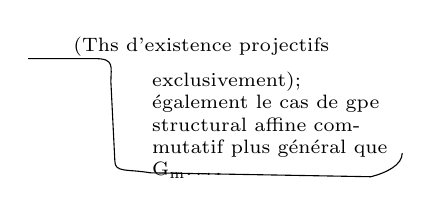
\begin{tikzpicture}[every node/.style={anchor=north west,font=\scriptsize,align=left}]
\node[text width=4cm] at (0,0) {(Ths d'existence projectifs};
\node[text width=3.2cm] at (1,-.45) {exclusivement\deleted{\unsure{)}}; également le cas de gpe structural affine commutatif plus général que $\mathrm G_{\mathrm m}$\ldots.};
\draw (-.45,-.4)--(.4,-.4)..controls (.65,-.4) and (.6,-.5)..(.6,-.7)--(.65,-1.7)..controls (.65,-1.85) and (.8,-1.8)..(1.1,-1.85)--(3.9,-1.9)..controls (4.1,-1.85) and (4.3,-1.75)..(4.3,-1.6);
\end{tikzpicture}}

\S\,17\quad Variantes de Picard.

\S\,1\deleted{\unsure{7}}8\quad Applications aux courbes

\S\,1\deleted{\unsure{8}}\unsure{9|8}\quad Formalisme des normes

\S\,\deleted{\unsure{19}}20\quad Invariants multiprojectifs de Mumford.

\figure{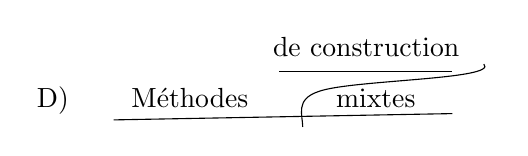
\begin{tikzpicture}[every node/.style={anchor=base west}]
\node at (0,0) {D)};\node at (1.2,0) {Méthodes};\node at (3.8,0) {mixtes};
\node at (3,.65) {\inserted{de construction}};
\draw (1.1,-.16)--(5.4,-.08);\draw (3.2,.45)--(5.4,.45);
\draw (5.8,.55)..controls (6,.35) and (4.1,.35)..(3.7,.2)..controls (3.4,.1) and (3.5,-.1)..(3.5,-.25);
\end{tikzpicture}}

\S\,2\deleted{0}1\quad Cas de représentabilité de $\mathrm P\underline{\mathrm{ic}}$, $\mathrm P\underline{\mathrm i\unsure{\mathrm c|\mathrm e}}^{\unsure{0|o|\circ}}$, $\unsure{-|\deleted{\mathrm P}}\mathrm P\underline{\mathrm{ic}}_{X}^{\tau}$ \ldots

(y compris le cas de Mumford utilisant \S\,\deleted{\unsure{19}}20).

\S\,21\quad Cas de représentabilité des foncteurs $\prod_{\deleted{X}Y/S}X/Y$ etc.

(\unsure{ths|Ths} du type Matsumura).

\noindent\rule{\linewidth}{.3pt}

NB.\quad On suppose \unsure{connues|connus} toutes les \unsure{gén.} fonctorielles (topologies, descente faisceaux, \unsure{quotients|quotient}) ; à rappeler au besoin dans $\unsure{0|O}_{\underline{\overline{\mathrm V}}}$.

\noindent\rule{\linewidth}{.3pt}

\uline{Manquent} :

\figure{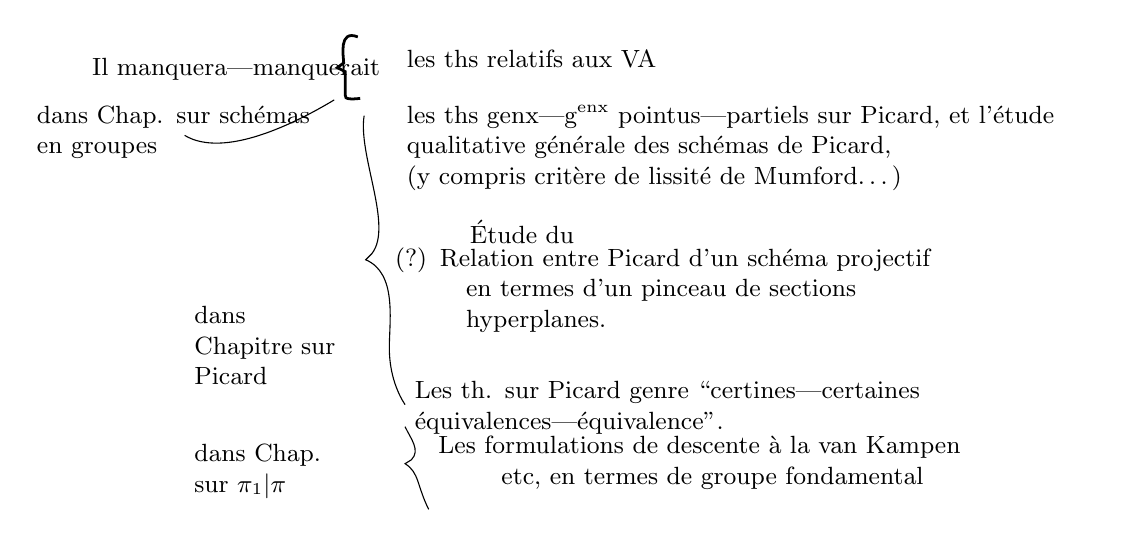
\begin{tikzpicture}[every node/.style={anchor=north west,align=left,font=\small}]
\node at (.7,0) {\deleted{Il \unsure{manquera|manquerait}}};
\node[text width=3.6cm] at (0,-.6) {dans Chap. sur schémas\\en groupes};
\node at (4.7,.1) {les ths relatifs aux VA};
\node[text width=8.3cm] at (4.7,-.6) {les ths \unsure{genx|g\textsuperscript{enx}} \unsure{pointus|partiels} sur Picard, et l'étude\\qualitative générale des schémas de Picard,\\(y compris critère de lissité de Mumford\ldots)};
\draw[line width=1pt] (4.2,.15)..controls (3.95,.25) and (4.02,-.1)..(4.02,-.18)--(3.94,-.24)--(4.04,-.29)--(4.04,-.59)..controls (4.02,-.65) and (4.15,-.64)..(4.23,-.63);
\draw (2,-1.1)..controls (2.5,-1.4) and (3.4,-.95)..(3.9,-.65);
\node[text width=2.2cm] at (2,-3.15) {dans\\Chapitre sur\\Picard};
\draw (4.28,-.85)..controls (4.2,-1.35) and (4.65,-2.25)..(4.38,-2.6)--(4.3,-2.68)..controls (4.7,-2.85) and (4.6,-3.45)..(4.6,-3.8)..controls (4.6,-4.15) and (4.72,-4.4)..(4.8,-4.52);
\node at (5.5,-2.05) {\inserted{Étude du}};
\node[text width=8.8cm] at (4.55,-2.4) {(?) \deleted{\unsure{Relation} entre} Picard d'un schéma projectif\\\hspace*{.9cm}en termes d'un pinceau de sections\\\hspace*{.9cm}hyperplanes.};
\node[text width=8.4cm] at (4.8,-4.1) {Les th. sur Picard genre ``\unsure{certines|certaines} \unsure{équivalences|équivalence}''.};
\node[text width=2.4cm] at (2,-4.9) {dans Chap.\\sur $\unsure{\pi_1|\pi}$};
\draw (4.8,-4.8)..controls (4.87,-4.95) and (5,-5.1)..(4.88,-5.22)--(4.8,-5.27)..controls (4.98,-5.38) and (4.95,-5.55)..(5.1,-5.85);
\node[text width=8.2cm] at (5.1,-4.8) {Les formulations de descente à la van Kampen\\\hspace*{.8cm}etc, en termes de groupe fondamental};
\end{tikzpicture}}
% archive sheet number: 4
